\section{模型检验}
\subsection{敏感性分析}
在模型建立之后,需要对模型进行敏感性分析。敏感性分析(sensitivity analysis)是指从定量分析的角度研究有关因素发生某种变化对某一个或一组关键指标影响程度的一种不确定分析技术。

具体分析步骤如下:
\begin{itemize}
	\item 确定指标
	敏感性分析的对象是具体的技术方案及其反映的经济效益。因此,技术方案的某些经济效益评价指标
	\item 计算该技术方案的目标值
	一般将在正常状态下的经济效益评价指标数值,作为目标值。
\end{itemize}

敏感性分析结果如图\ref{p-15}。
\begin{figure}[h]
	\centering
	\begin{minipage}[b]{0.45\linewidth}
		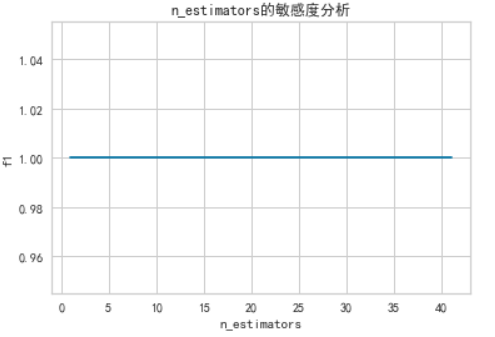
\includegraphics[width=1\textwidth]{敏感性分析1.png}		
	\end{minipage}
	\begin{minipage}[b]{0.45\linewidth}
		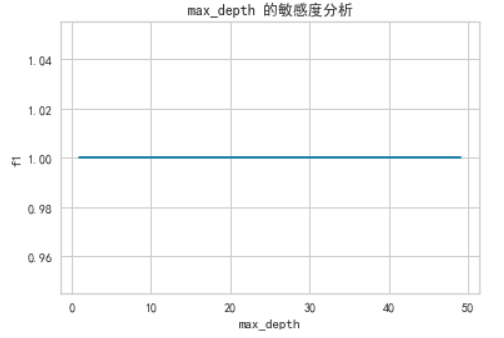
\includegraphics[width=1\textwidth]{敏感性分析2.png}
	\end{minipage}
	\setlength{\abovecaptionskip}{3pt}%caption与表格之间的距离
	\caption{逻辑回归敏感性分析结果展示}
	\label{p-15}
\end{figure}

\subsection{差异性分析}
图中展示模型检验的结果表 分析了相关系数的正负向以及相关性程度进一步推出了其中的差异性若呈现数绝对值值较大,说明其两变量存在相关性,否则不相关

\begin{figure}[!h]
	\centering
	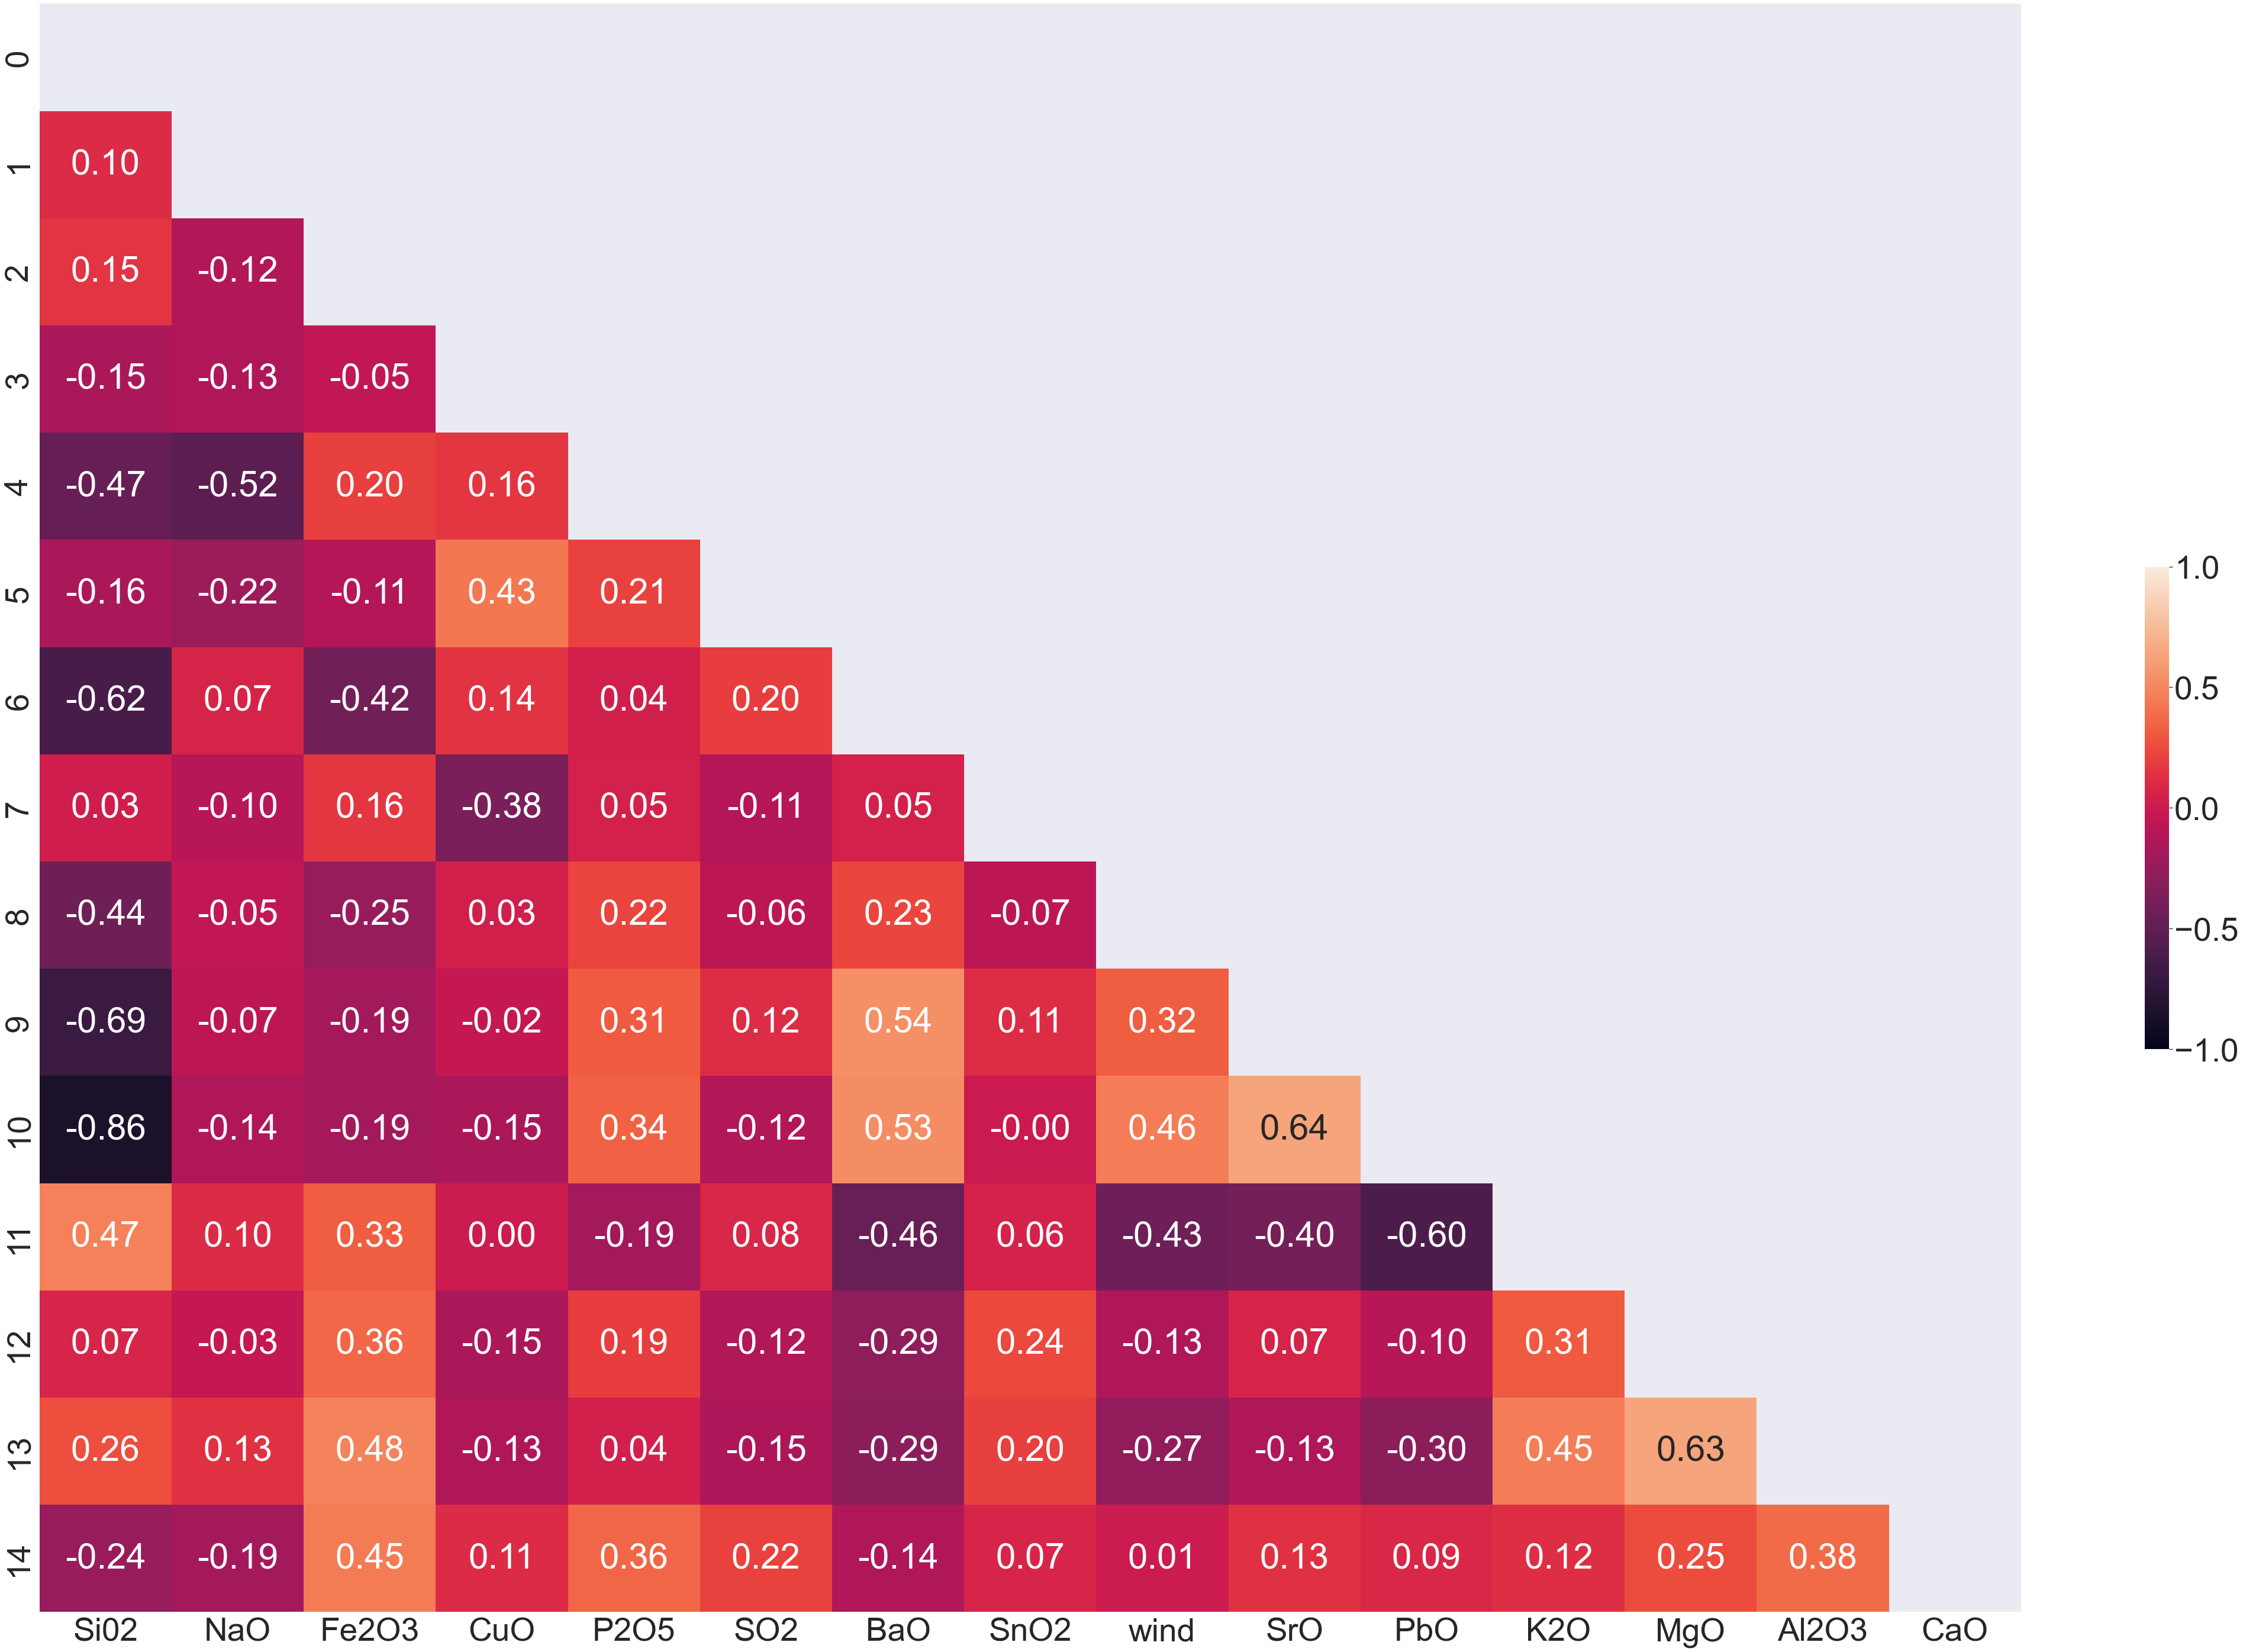
\includegraphics[width=0.6\textwidth]{s4.png}
	\setlength{\abovecaptionskip}{3pt}%caption与表格之间的距离
	\caption{相关系数}
	\label{p-17}
\end{figure}

图\ref{p-17}展示了热力图的形式展示了相关系数的值,主要通过颜色深浅去表示值的大小。